\chapter{Desarrollo} \label{development}
En este capítulo se presentan las actividades realizadas durante el desarrollo del proyecto correspondientes al período de pasantías Abril-Septiembre 2018. El proyecto inicialmente tenía planteado el desarrollo de cuatro módulos:
\begin{enumerate}
	\item Módulo de administración de cadenas, tiendas, zonas, productos y categorías: El alcance inicial de este módulo consistía en el desarrollar la interfaz gráfica para crear, editar y eliminar los registros de cada una de estas entidades, asignar tiendas a cadenas, asignar productos a categorías, y desarrollar la funcionalidad para listar los registros de productos con mecanismo de búsqueda. Para el desarrollo de este módulo se tuvo una duración de 1 Sprint \ref{sprint} sin embargo no se logró completar todo el módulo en ese tiempo, y se quedó por desarrollar las entidades tiendas y zonas para el último Sprint ya que las entidades de mayor relevancia ya estaban implementadas, pero como se tuvo otros retrasos durante el desarrollo del proyecto, el Dueño del Producto decidió dejar estas entidades para una próxima versión de la aplicación, debido a que con las entidades implementadas se podían utilizar todas las funcionalidades planificadas.
    \item Módulo de administración de precios: Este módulo incluye la interfaz de creación, edición y eliminación de registros, el desarrollo de un mecanismo para importar los precios en lote usando un archivo en formato Microsoft Excel y de igual manera importar por lote mediante webservice desde una fuente externa en formato JSON, sin embargo ésta última no se realizó ya que este módulo estaba planificado para ser desarrollado en 1 Sprint, y no se tuvo el tiempo suficiente para desarrollar esta funcionalidad, por lo que el Dueño del Producto decidió dejarlo para una próxima versión ya que con un método de importación de precios bastaba para esta versión de la aplicación.
	\item Módulo de generación de reportes: Para este módulo se planteó el desarrollo de la funcionalidad de generar reportes comparativos para: 
    \begin{itemize}
        \item Gráfico de dispersión de precios / categorías.
        \item Gráfico de barras para un producto seleccionado separando precio normal y oferta.
        \item Gráfico tipo box-plot para el histórico de precios de un producto.
	\end{itemize}
	Implementar un mecanismo automático para generar reportes de manera frecuente y enviar alertas de correo con el resultado, y finalmente un mecanismo para exportar los reportes en un formato tipo tabla en Microsoft Excel, sin embargo estas dos últimas funcionalidades se decidieron dejar para una próxima versión del sistema, ya que el desarrollo de la primera funcionalidad tomó más tiempo del pensado, debido a su complejidad.
	\item Módulo de preferencias para usuario: Este módulo no se desarrolló, debido a que el mismo tenía directa relación con las dos últimas funcionalidades del módulo anterior y al no desarrollarlas, este módulo no tenía sentido. 
\end{enumerate}
    El proyecto se dividió en 3 Fases :
\begin{itemize}
   \item Fase de Inducción, en la cual se hace la introducción del proyecto, el pasante se familiarizó con las herramientas y tecnologías necesarias para realizar el proyecto.
   \item Fase de Desarrollo la cual se dividió en 5 Sprints, en esta fase se hace la implementación de los diferentes módulos de la aplicación.
   \item Fase de Documentación en la cual se realiza parte de la documentación necesaria para la aplicación.
\end{itemize}
A continuación, se explicará en detalle en qué consiste cada Fase.

\section{Inducción}
Durante esta Fase el pasante realizó un proceso de familiarización con la empresa junto con el estudio de herramientas y lenguajes de trabajo que fueron empleados a lo largo del desarrollo del proyecto.
Realizó varios cursos tutoriales (Umbraco Course level 1, Learn ASP.NET MVC de Microsoft Virtual Academy, entre otros),  y utilizó recursos (guía de Umbraco) que la empresa proporcionó para tener los conocimientos necesarios para llevar a cabo el proyecto. Además investigó sobre herramientas como: ASP.NET, SQL Server, Highcharts y Visual Studio.

La duración de esta fase fue de una semana, sin embargo, el pasante tuvo que mantenerse en constante búsqueda de recursos e investigar sobre la marcha sobre herramientas o conceptos nuevos, los cuales se fueron necesitando en el camino. Todo este proceso fue sumamente útil y de gran aprendizaje ya que la mayoría de las herramientas utilizadas para el desarrollo del proyecto eran nuevas y muchos de los conceptos se investigaron a profundidad.

\section{Desarrollo}
La Fase de desarrollo de la aplicación se realizó en cinco Sprints, los cuales tuvieron una duración en total de 17 semanas continuas. A continuación una descripción del trabajo realizado en cada uno.

\subsection{Primer Sprint}
Durante este Sprint se hizo el análisis y definición de los requerimientos de la aplicación, los cuales eran primero definir el alcance inicial de la aplicación (ver Figura \ref{fig:cu_admin_inicial} y Figura \ref{fig:cu_retailer_inicial}), definir la arquitectura a utilizar y por último la estructura de la base de datos. El pasante inició la familiarización de la versión actual de CPI junto con el dueño del producto para resolver las posibles dudas de la funcionalidad, o conceptos necesarios para entender la aplicación. Además se creó el repositorio de Git, el proyecto de Visual Studio y el sitio de Umbraco, y por último el Dueño del producto sugirió dos posibles plantillas de HTML que podrían ser utilizadas para las vistas de la aplicación y el pasante eligió la que era más adecuada visual y funcionalmente para la misma.
\vskip 0.5cm
\textbf{Actividades realizadas:}
\begin{itemize}
  \item Familiarización con la versión original de CPI. Esta actividad consistió principalmente en reuniones con el dueño del producto para aclarar dudas con respecto a los conceptos necesarios para entender la aplicación y sus funcionalidades.
  \item Elegir la arquitectura de la aplicación. El pasante junto con el Dueño del Producto decidieron utilizar el modelo de 4+1 Vistas de Philippe Kruchten \cite{vistasKruchten}, el cual  propone que un sistema software se ha de documentar y mostrar con 4 vistas bien diferenciadas y que tienen que relacionar entre sí con una vista más, que es la denominada vista “+1”. Estas vistas son: vista lógica, vista de procesos, vista de despliegue, vista física y la vista “+1” llamada vista de escenario.
  \item Definir los actores del sistema. En principio se definieron dos actores principales para la aplicación, \textit{Admin} (el administrador del sistema) y \textit{Retailer} (representantes de cadenas).
  \item Realizar una matriz de permisología de las funcionalidades de la aplicación. Lo que el pasante realizó fue listar todas las posibles funciones de cada uno de los módulos de aplicación y definir cuáles eran los permisos que tendrán cada uno de los actores.
  \item Elegir las entidades de la aplicación. El pasante basándose en la primera versión de la aplicación y junto el dueño del producto tomaron la decisión de cuáles serían las entidades que se manejarían desde la base de datos de Umbraco (cadenas) y cuáles en la base de datos de SQL Server (tiendas, zonas, productos, precios y categorías).
  \item Rediseñar la base de datos. Luego de decidir cuáles eran las entidades a trabajar en la base de datos de SQL Server el pasante junto con el Dueño del Producto decidieron cuál podría ser la nueva estructura de la base de datos. A continuación se muestra el Diagrama de la versión original de CPI (ver Figura \ref{fig:er_viejo}) y el Diagrama ER de la versión 2 de CPI (ver Figura \ref{fig:er_nuevo})
  \item Crear el proyecto en Visual Studio. 
  \item Crear el repositorio de Git. Para el proyecto se creó un repositorio llamado CPI el cual se utilizó para el control de versiones del proyecto. Para utilizar correctamente el repositorio el pasante tuvo que refrescar los comandos.
  \item Crear el sitio de Umbraco.
  \item Elegir la plantilla a utilizar para las vistas de la aplicación. El pasante junto con el Dueño del Producto eligieron entre dos posibles plantillas, la elegida fue la que más se acopló a las necesidades de la aplicación.
  \item Investigar sobre Datatables ya que fue el pluggin (complemento) elegido por el Dueño del Producto para manejar dinámicamente las tablas.
  \item Listar las vistas que tendrá la aplicación, según los módulos que se eligieron como alcance inicial.
\end{itemize}

        
\textbf{Duración:} 2 semanas.

       \begin{figure}[H]
       \begin{center}
       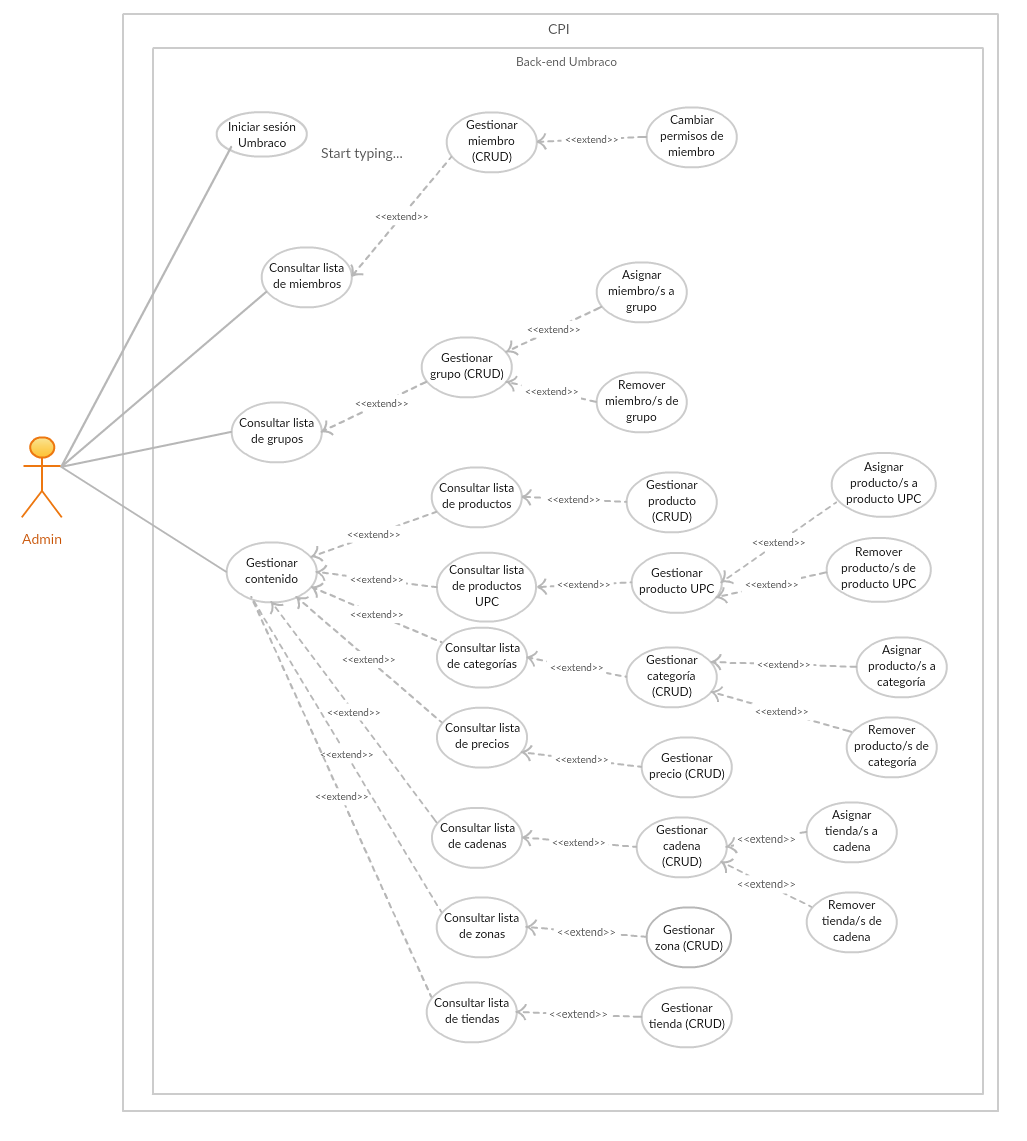
\includegraphics[width=\textwidth]{cu_admin_inicial.png}
       \caption{Diegrama Diagrama de Casos de Uso para Admin inicial. Elaboración propia.}
       \label{fig:cu_admin_inicial}
       \end{center}
       \end{figure}

       \begin{figure}[H]
       \begin{center}
       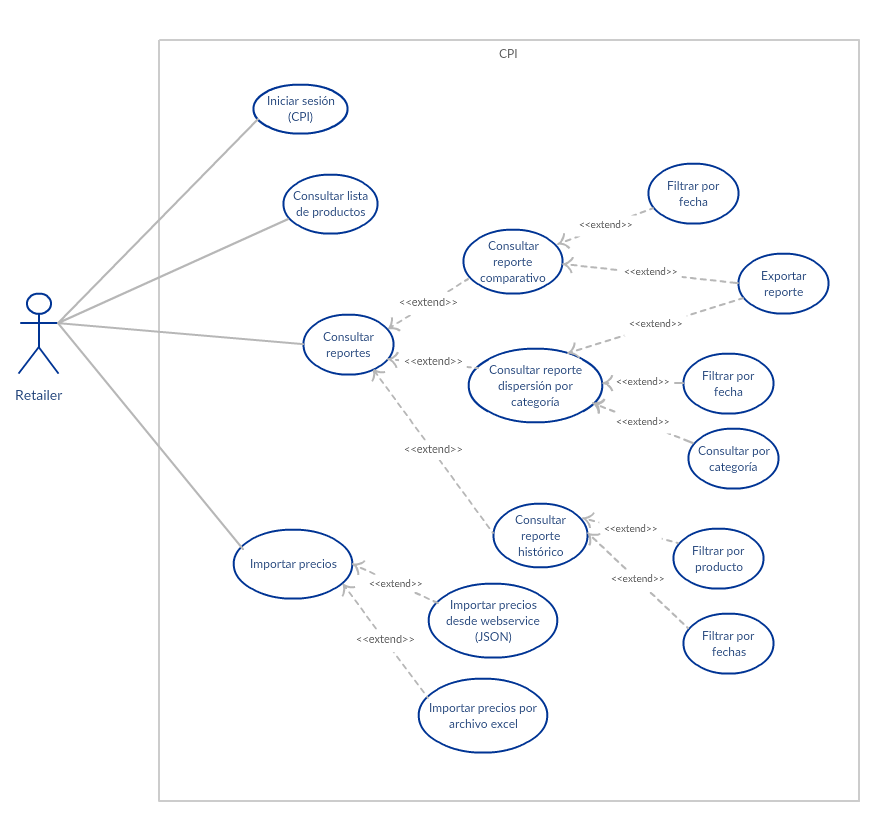
\includegraphics[width=\textwidth]{cu_retailer_inicial.png}
       \caption{Diagrama de Casos de Uso para Retailer inicial. Elaboración propia.}
       \label{fig:cu_retailer_inicial}
       \end{center}
       \end{figure}

    
       \begin{figure}[H]
       \begin{center}
       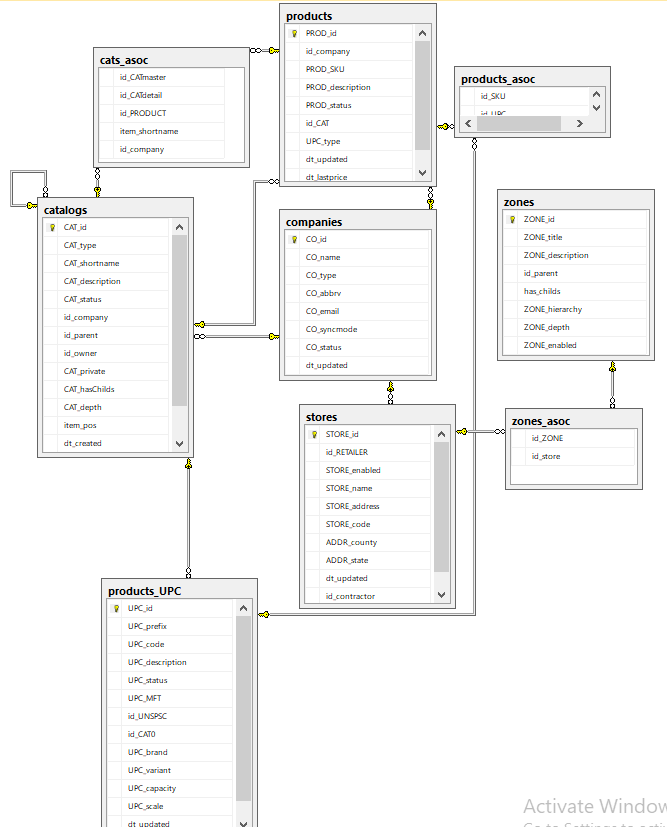
\includegraphics[width=\textwidth]{er_viejo.png}
       \caption{Diegrama ER de la base de datos de la versión 1 de CPI.}
       \label{fig:er_viejo}
       \end{center}
       \end{figure}

       \begin{figure}[H]
       \begin{center}
       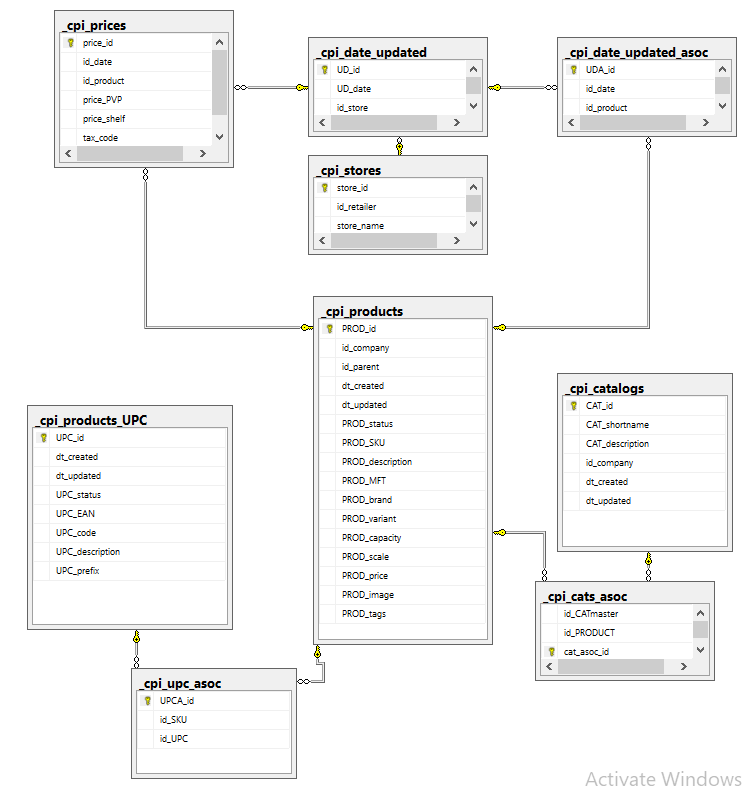
\includegraphics[width=\textwidth]{er.png}
       \caption{Diagrama de la base de datos de la nueva versión de CPI.}
       \label{fig:er_nuevo}
       \end{center}
       \end{figure}


\subsection{Segundo Sprint (Módulo de Administración de cadenas, productos y categorías)}
Durante este Sprint se implementó la funcionalidad para el manejo de las principales entidades de la aplicación: cadenas, productos y categorías, en la cual se desarrolló una interfaz gráfica en el back end de Umbraco usando un paquete llamado Fluidity para el manejo de estas entidades en la base de datos. Se definieron los Doctypes (tipos de documento) y Datatypes (tipos de datos) para crear el contenido en Umbraco. Se inició el desarrollo de las vistas de la aplicación. Y por último se empezó la implementación para la vista de listado de productos.
\vskip 0.5 cm
\textbf{Actividades realizadas:}
\begin{itemize}
   \item Definir los Doctypes para las entidades principales. El pasante definió las propiedades que tendrían cada una de las entidades que se encuentran en Umbraco (ver en el Anexo \ref{das} la Sección 8.2).
   \item Definir los Datatypes que usan las entidades principales. El pasante creo tipos de datos necesarios para las propiedades de las entidades a usarse en Umbraco (ver en el Anexo \ref{das} la Sección 8.1).
   \item El Dueño del producto realizó una instalación local de la versión 1 de la aplicación CPI para que el pasante pudiera revisar a fondo la funcionalidad actual y además revisar el código fuente y la base de datos para ayudar al desarrollo de la nueva versión de la aplicación.
   \item El Dueño del Producto propuso dos paquetes de Umbraco para gestionar los datos de la base de datos de SQL Server (Fluidity o UI-Matic) y el pasante investigó sobre ambos y se decidió elegir Fluidity ya que era un paquete desarrollado más recientemente y además era compatible con la versión de Umbraco utilizada para el desarrollo de la aplicación. Luego se desarrolló la interfaz de Fluidity para creación, edición y eliminación de registros de las entidades que se guardan en la base de datos de SQL Server, para de esta manera poder manejar los registros desde el back end de Umbraco. Para poder realizar la interfaz y poder manejar correctamente los datos de las tablas de la base de datos, en algunos casos se tuvo que agregar un campo adicional a la tabla y el mismo se tomaba como clave primaria, ya que estas tablas tenían dos claves primarias y Fluidity no manejaba correctamente este tipo de casos.
   \item Se desarrollaron las principales partials views (vistas parciales) que tienen en común todas las vistas de la aplicación, como por ejemplo la barra de navegación y la barra lateral.
   \item Se realizó la implementación de la vista y la funcionalidad para listar los productos por cadena, y esto se hizo utilizando Datatables.
\end{itemize}
\textbf{Duración:} 3 semanas.


\subsection{Tercer Sprint (Módulo de Generación de Reportes)}
En este Sprint se desarrolló parte de la funcionalidad de generación de reportes comparativos. Este módulo cuenta con tres tipos de reportes, sin embargo únicamente se pudieron desarrollar dos de ellos (reporte de comparación de precios de un producto en distintas cadenas, y reporte histórico de precios de un producto) ya que el tiempo de desarrollo de los gráficos usando la herramienta Highcharts tomó más tiempo del que se tenía planificado porque al ser una herramienta que el pasante no utilizó anteriormente se necesitó de tiempo para aprender a utilizarla y luego para poder traer los datos correctamente de la base de datos (los cuales son los que se ven reflejados en cada uno de los gráficos) se necesitó de la traducción, entendimiento y mejora considerable del código de la versión antigua y esto se hizo bastante engorroso ya que los scripts no estaban bien documentados.
\vskip 0.5cm
\textbf{Actividades realizadas:}
\begin{itemize}
   \item Elección de la herramienta para hacer los gráficos necesarios para los reportes. El Dueño del Producto propuso dos herramientas para la generación de los gráficos, la primera era Chartjs que es de licencia gratuita y la segunda se llama Highcharts la cual es de licencia paga. El pasante para realizar la elección de la herramienta, realizó ejemplos de gráficos usando ambas opciones para comparar complejidad, facilidad de conseguir recursos y ejemplos para ayudar con el desarrollo, entre otras cosas, y llegó a la conclusión que la herramienta más apta para ser usada en la aplicación era Highcharts ya que contaba con todos los tipos de gráficos necesarios para la aplicación (Chartjs no contaba con gráfico boxplot) y cuenta con mayor documentación y ejemplos en los que se podía apoyar para el desarrollo de los gráficos. 
   \item Revisión de la documentación y la Referencia API de JavaScript de Highcharts para poder comenzar con el desarrollo de los gráficos para los reportes.
   \item Implementación del reporte de comparación de precios de un producto en común entre distintas cadenas. Este reporte se divide en dos partes, la primera es un gráfico de barras en el que se ven reflejados el precio normal y el precio por oferta del producto en las distintas cadenas, y la segunda parte es una tabla con información más detallada del producto (precio PVP, precio oferta, IVA del producto y número de tiendas dentro de la cadena en la que se encuentra disponible dicho producto).
   \item Implementación del reporte histórico de un producto en un período de tiempo, para esto se realizó un gráfico boxplot en el que se muestra una caja por fecha en el que esté registrado el precio de ese producto dentro del período elegido.
\end{itemize}

\textbf{Duración:} 4 semanas.

\subsection{Cuarto Sprint (Continuación con el Módulo de Generación de Reportes)}

En este Sprint se realizó el reporte de precios de productos por categorías (gráfico de dispersión) que faltó por realizar en el Sprint anterior, y además se corrigieron detalles de los otros dos reportes ya implementados.
\vskip 0.5cm
\textbf{Actividades realizadas:}
\begin{itemize}
   \item Se agregó a la interfaz de Fluidity que ya se encontraba implementada la función para asignar productos a categorías.
   \item Agregar enlace de la tabla de productos al reporte de comparación de precios. A la lista de todos los productos se le agregó un enlace desde el código SKU del producto hacia el reporte de comparación de precios de productos de diferentes cadenas.
   \item Implementación del reporte de precios de productos por categorías. Primero para comenzar con la implementación se realizó un boceto con datos ficticios del gráfico de dispersión para que el pasante se familiarizara con la complejidad de este tipo de gráficos. Luego se realizó la traducción, mejora y entendimiento del código de la versión antigua de la aplicación para manejar los datos que se encuentran en la base de datos y reflejarlos en el gráfico.
   \item Se inició la construcción del diccionario de Umbraco con las palabras estáticas y que se repiten en cada una de las vistas de la aplicación.
   \item Se corrigieron detalles de los reportes anteriores. Para el reporte de comparación de precios de un producto se corrigió el formato de la fecha (pasó  de utilizarse “mm/dd/yyyy” a el formato ISO “yyyymmdd”) de igual manera para el reporte histórico, se arreglaron detalles del código de HTML y eficiencia de los controladores para traer la información de la base de datos.
\end{itemize}

\textbf{Duración:} 4 semanas.


\subsection{Quinto Sprint (Módulo de Administración de Precios y Corrección de estructura del proyecto)} 
Este es el último Sprint de desarrollo, en el mismo se implementó el módulo de administración de precios de productos. El alcance inicial de este módulo era realizar la interfaz gráfica para la creación, edición y eliminación de registros, importar precios por lote mediante un archivo en formato Microsoft Excel e importar mediante webservice desde una fuente externa en formato JSON, sin embargo la última funcionalidad no se pudo desarrollar ya que durante el sprint el pasante se dió cuenta de que había un error en la estructura, ya que la misma no estaba siguiendo el patrón MVC que se debía tener en la solución de Visual Studio. Este error en la estructura fue debido a la falta de comunicación entre el pasante y el Dueño del Producto sobre aspectos técnicos del proyecto, y para corregir este inconveniente se tomó tiempo del Sprint por lo que no alcanzó para completar el módulo y se decidió dejar esta funcionalidad para más adelante.
\vskip 0.5cm
\textbf{Actividades realizadas:}
\begin{itemize} 
   \item Se implementó la autenticación, inicio y cierre de sesión para el front end de la aplicación. Para esto primero se definen los permisos de usuarios, en este caso, para el alcance de la aplicación únicamente se tiene el usuario \emph{retailer}, y se creó un grupo de miembro en el back end de Umbraco en la sección Members llamado \emph{cpi user}, luego se desarrolló la vista para el iniciar y cerrar sesión.
   \item Se desarrolló la interfaz gráfica para creación, edición y eliminación de registros usando el paquete de Umbraco Fluidity para poder manejar esta entidad directo de la plataforma, modificando directamente la base de datos de SQL Server.
   \item Se realizó la implementación para importar por lote los precios desde un archivo en formato Microsoft Excel.
   \item El código de la aplicación pasó a revisión y de esta manera encontrar detalles de escritura y aplicar buenas prácticas de desarrollo. Por lo que se mejoraron nombres y declaraciones de variables, se agregaron mas comentarios para el entendimiento del código, y eliminación de librerías que no se usaban por las clases.
   \item Reorganización de controladores y vistas de la aplicación. Luego de revisar y corregir los errores encontrados, se consiguió un error en la estructura de la solución de Visual Studio, ya que no se estaba siguiendo el patrón MVC que se había escogido al principio de la pasantía. Por lo que para resolver esto, se organizaron los controladores y las vistas de la aplicación.
\end{itemize}

\textbf{Duración:} 4 semanas.
\vskip 0.5cm
A continuación se muestran los Diagramas de casos de Uso desarrollados al final de esta fase.

\begin{figure}[H]
    \begin{center}
    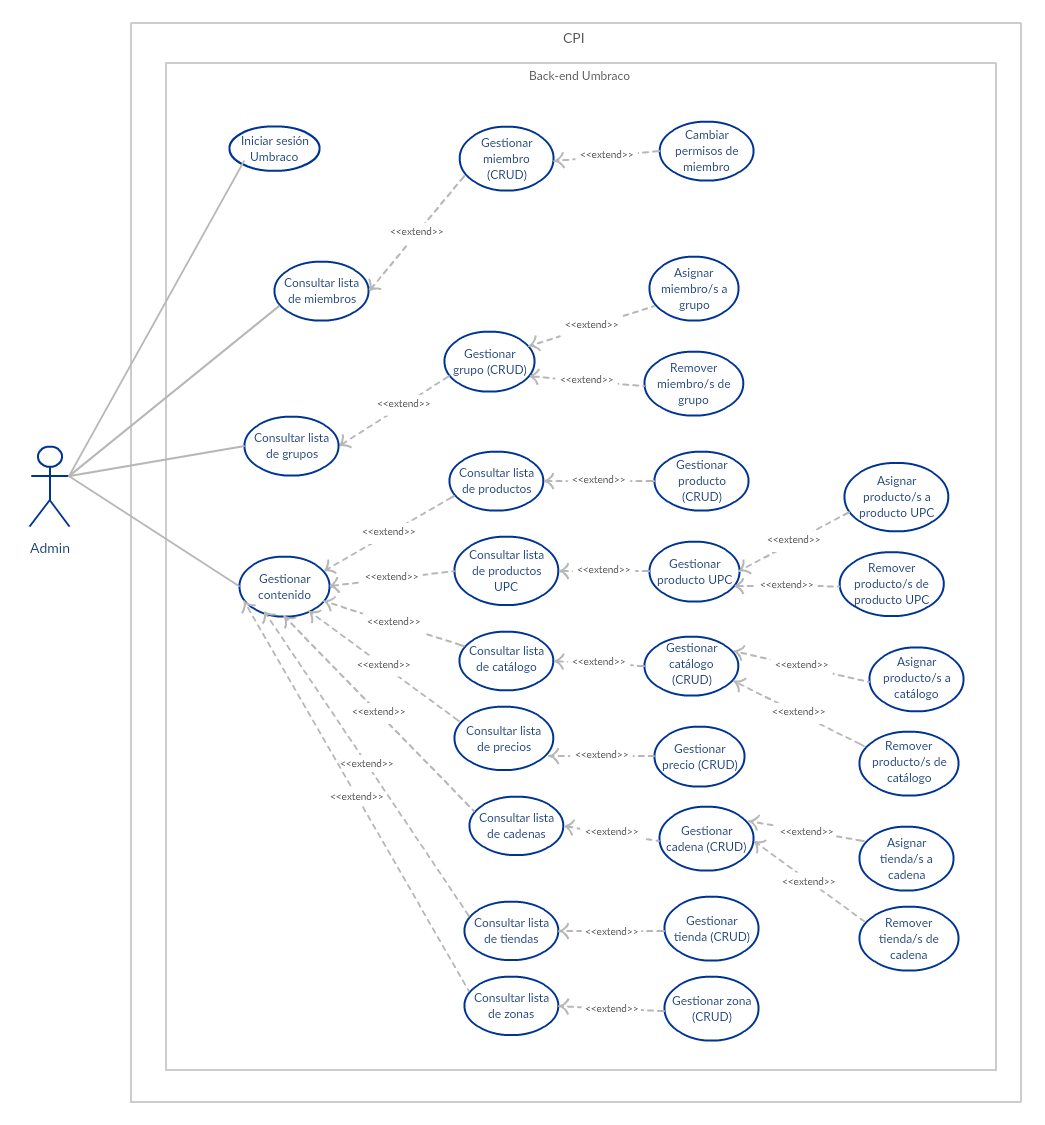
\includegraphics[width=\textwidth]{cu_admin.png}
    \caption{Diagrama de Casos de Uso desarrollados para el actor Admin. Elaboración propia.}
    \label{fig:cu_admin}
    \end{center}
\end{figure}

\begin{figure}[H]
    \begin{center}
    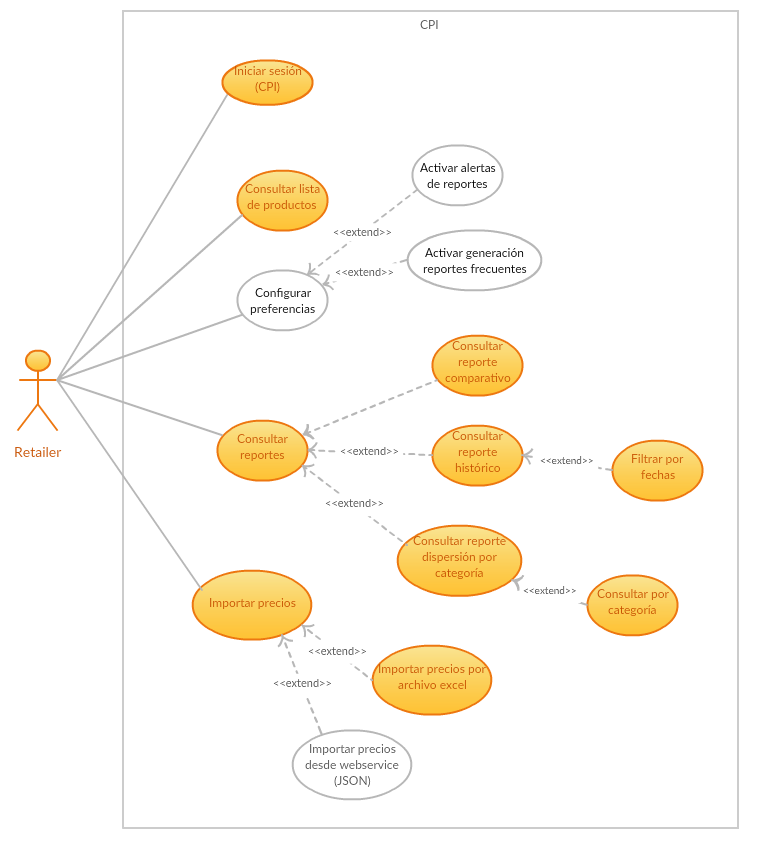
\includegraphics[width=\textwidth]{cu_retailer.png}
    \caption{Diagrama de Casos de Uso desarrollados para el actor Retailer. Elaboración propia.}
    \label{fig:cu_retailer}
    \end{center}
\end{figure}

\section{Documentación} \label{documentation}
Esta última fase del proyecto duró las últimas dos semanas del período de pasantía. Se realizó la documentación necesaria para la aplicación, se dejó expresado el estado final del sistema, se elaboraron los documentos de instalación de CPI y el Documento de Arquitectura de Software (ver Anexo \ref{das}) donde se detallan los componentes y casos de uso desarrollados de la aplicación.
